\documentclass{article}
%\usepackage[margin=1.0in]{geometry}
\usepackage{graphicx}

\title{Fractal Dimension in Time Varying Networks}

%\addtolength{\oddsidemargin}{1.0in}
%\addtolength{\evensidemargin}{1.0in}
%\addtolength{\textwidth}{1.75in}
%\addtolength{\topmargin}{0.3in}
%\addtolength{\textheight}{1.75in}

\begin{document}
\section{Introduction}

\section{Related Work}

\section{Experimental Details}


\subsection{Used Dataset}
The Dataset used for Analysis is obtained from here\footnote{http://www.sociopatterns.org/}.

\subsection{Experimental Methodology}
For a given network $G$ and box size $l_B$, a box is a set of nodes where all distances $l_{ij}$ between any two nodes i and j in the box are smaller than $l_B$. The minimum number of boxes required to cover the entire network $G$ is denoted by $N_B$. For $l_B$ = 1, $N_B$ is obviously equal to the size of the network $N$, while $N_B$ = 1 for $l_B \geq l_B^{max}$ , where $l_B^{max}$ is the diameter of the network (i.e. the maximum distance in the network) plus one.

The ultimate goal of all box-covering algorithms is to locate the optimum solution, i.e., to identify the minimum $N_B(l_B)$ value for any given box size $l_B$. We first demonstrate that this problem can be mapped to the graph coloring problem, which is known to belong to the family of NP-hard problems. This means that an algorithm that can provide an exact solution in a relatively short amount of time does not exist. This concept, though, enables us to treat the box covering problem using known optimization approximations. In order to find an approximation for the optimal
solution for an arbitrary value of $l_B$ we first construct a dual network $G'$, in which two
nodes are connected if the chemical distance between them in $G$ (the original network)
is greater or equal than $l_B$.
Vertex coloring is a well-known procedure, where labels (or colors) are assigned to
each vertex of a network, so that no edge connects two identically colored vertices. It
is clear that such a coloring in $G'$ gives rise to a natural box covering in the original
network $G$, in the sense that vertices of the same color will necessarily form a box since
the distance between them must be less than $l_B$. Accordingly, the minimum number
of boxes $N_B(G)$ is equal to the minimum required number of colors (or the chromatic
number) in the dual network $G'$, $\chi(G')$, which is a famous problem in traditional graph
theory.


\section{Experimental Results}
The plots for a 69-day Time Varying Real World Networks, divided into 10 groups each containg a 7-day set of plots, followed by the plot of variation of fractal dimension($d_B$) w.r.t. time($t$) in days are as follows:
\begin{figure}
\centering
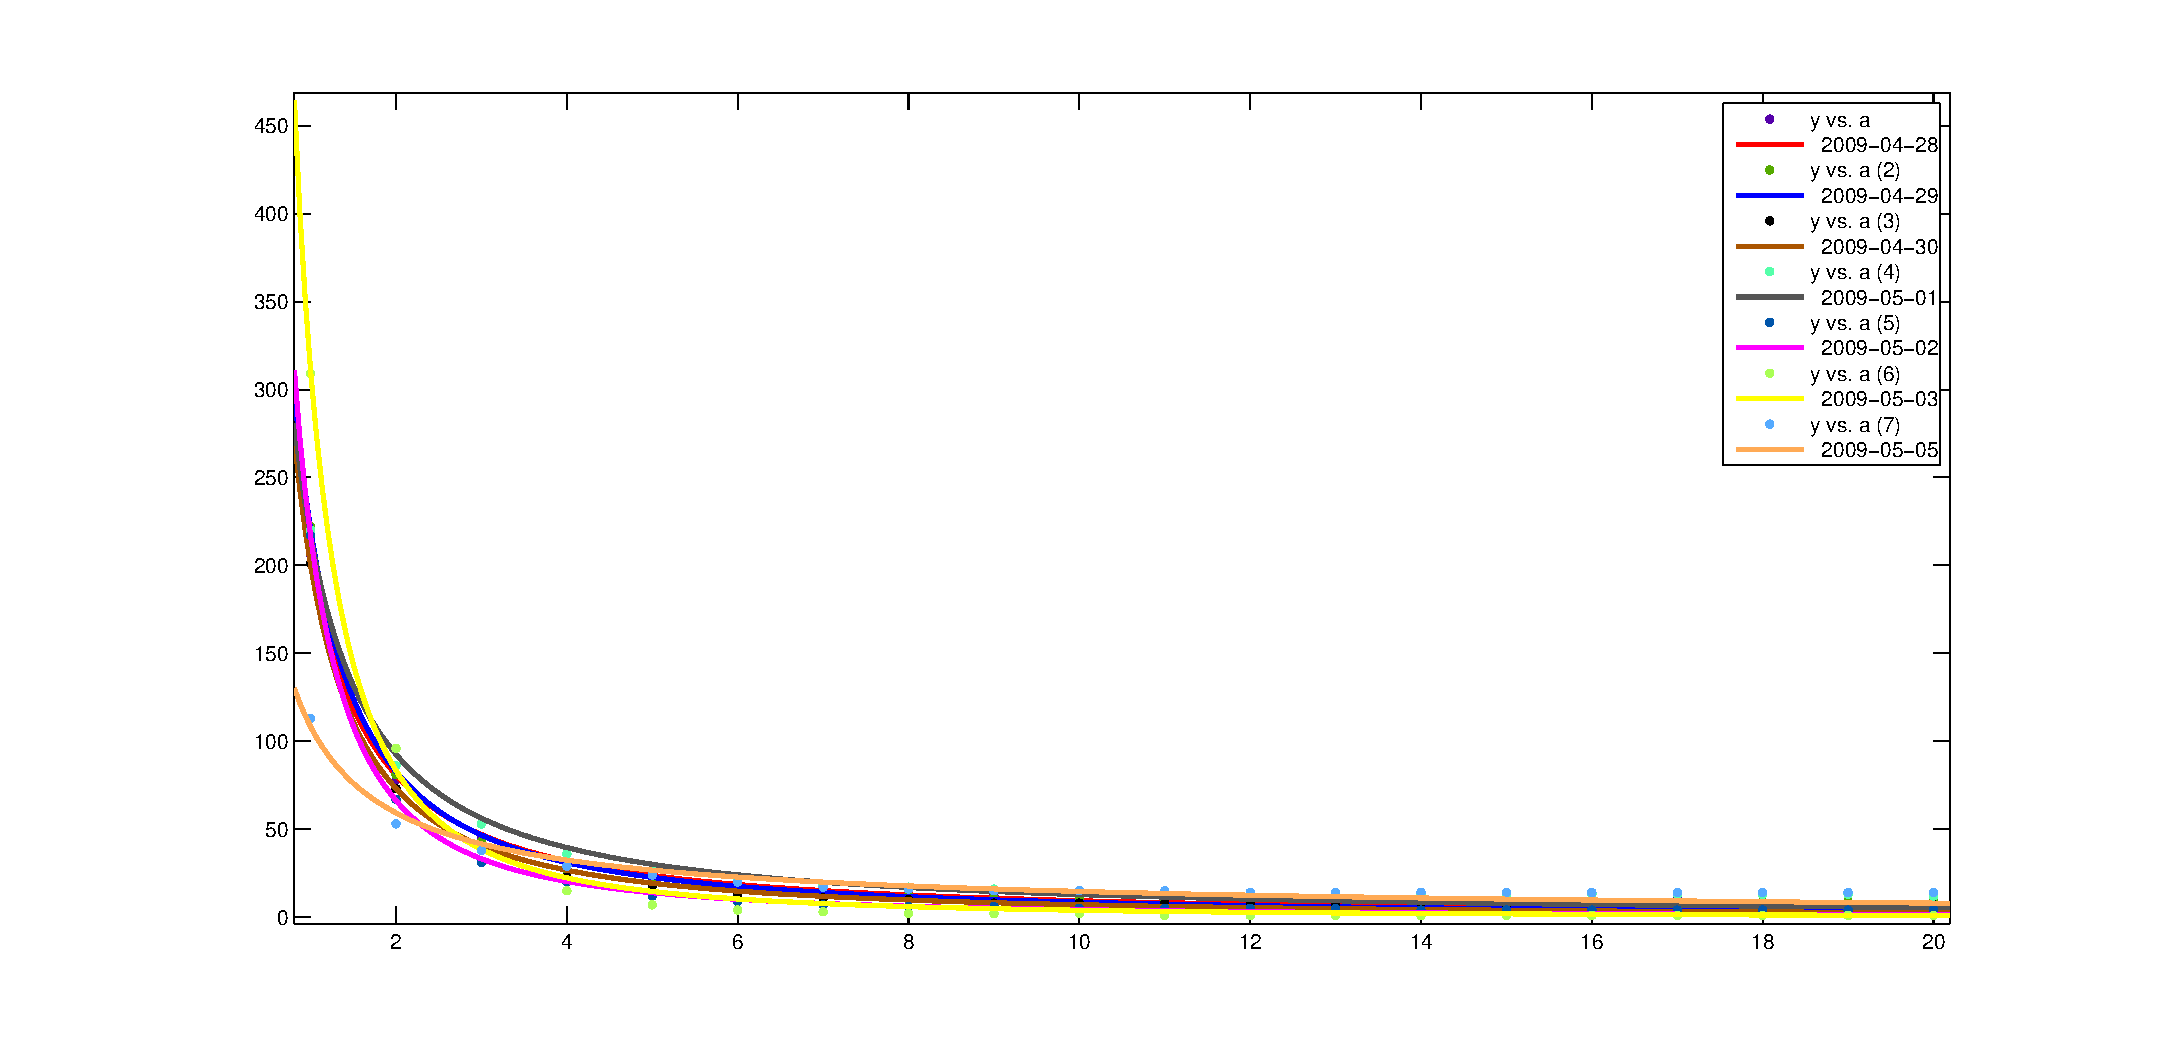
\includegraphics[scale=0.3]{plot1/plot1}
\caption{Plots of Number of boxes($N_B$) vs Length of Box($l_B$) for days 1-7.}
\end{figure}
\begin{figure}
\centering
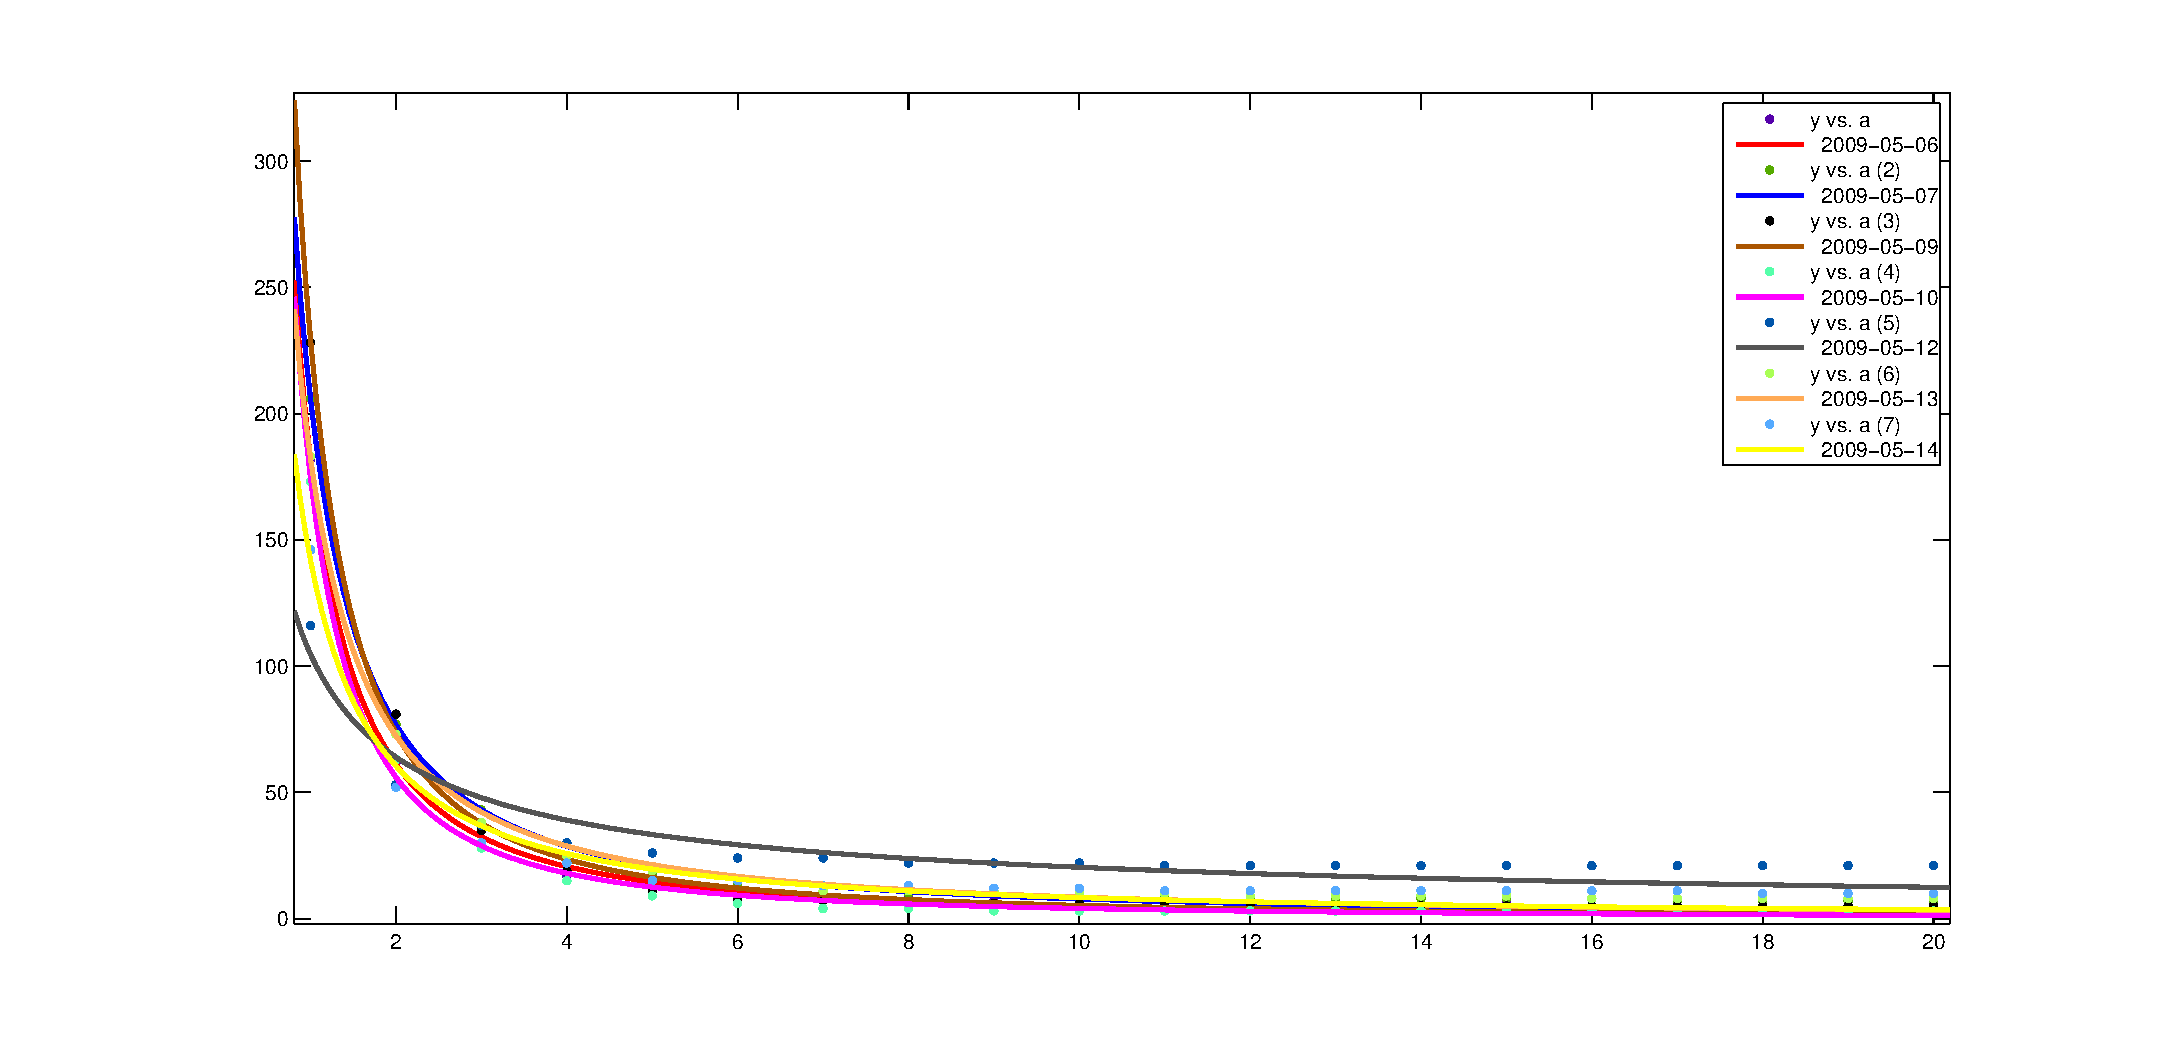
\includegraphics[scale=0.3]{plot2/plot2}
\caption{Plots of Number of boxes($N_B$) vs Length of Box($l_B$) for days 8-14.}
\end{figure}
\begin{figure}
\centering
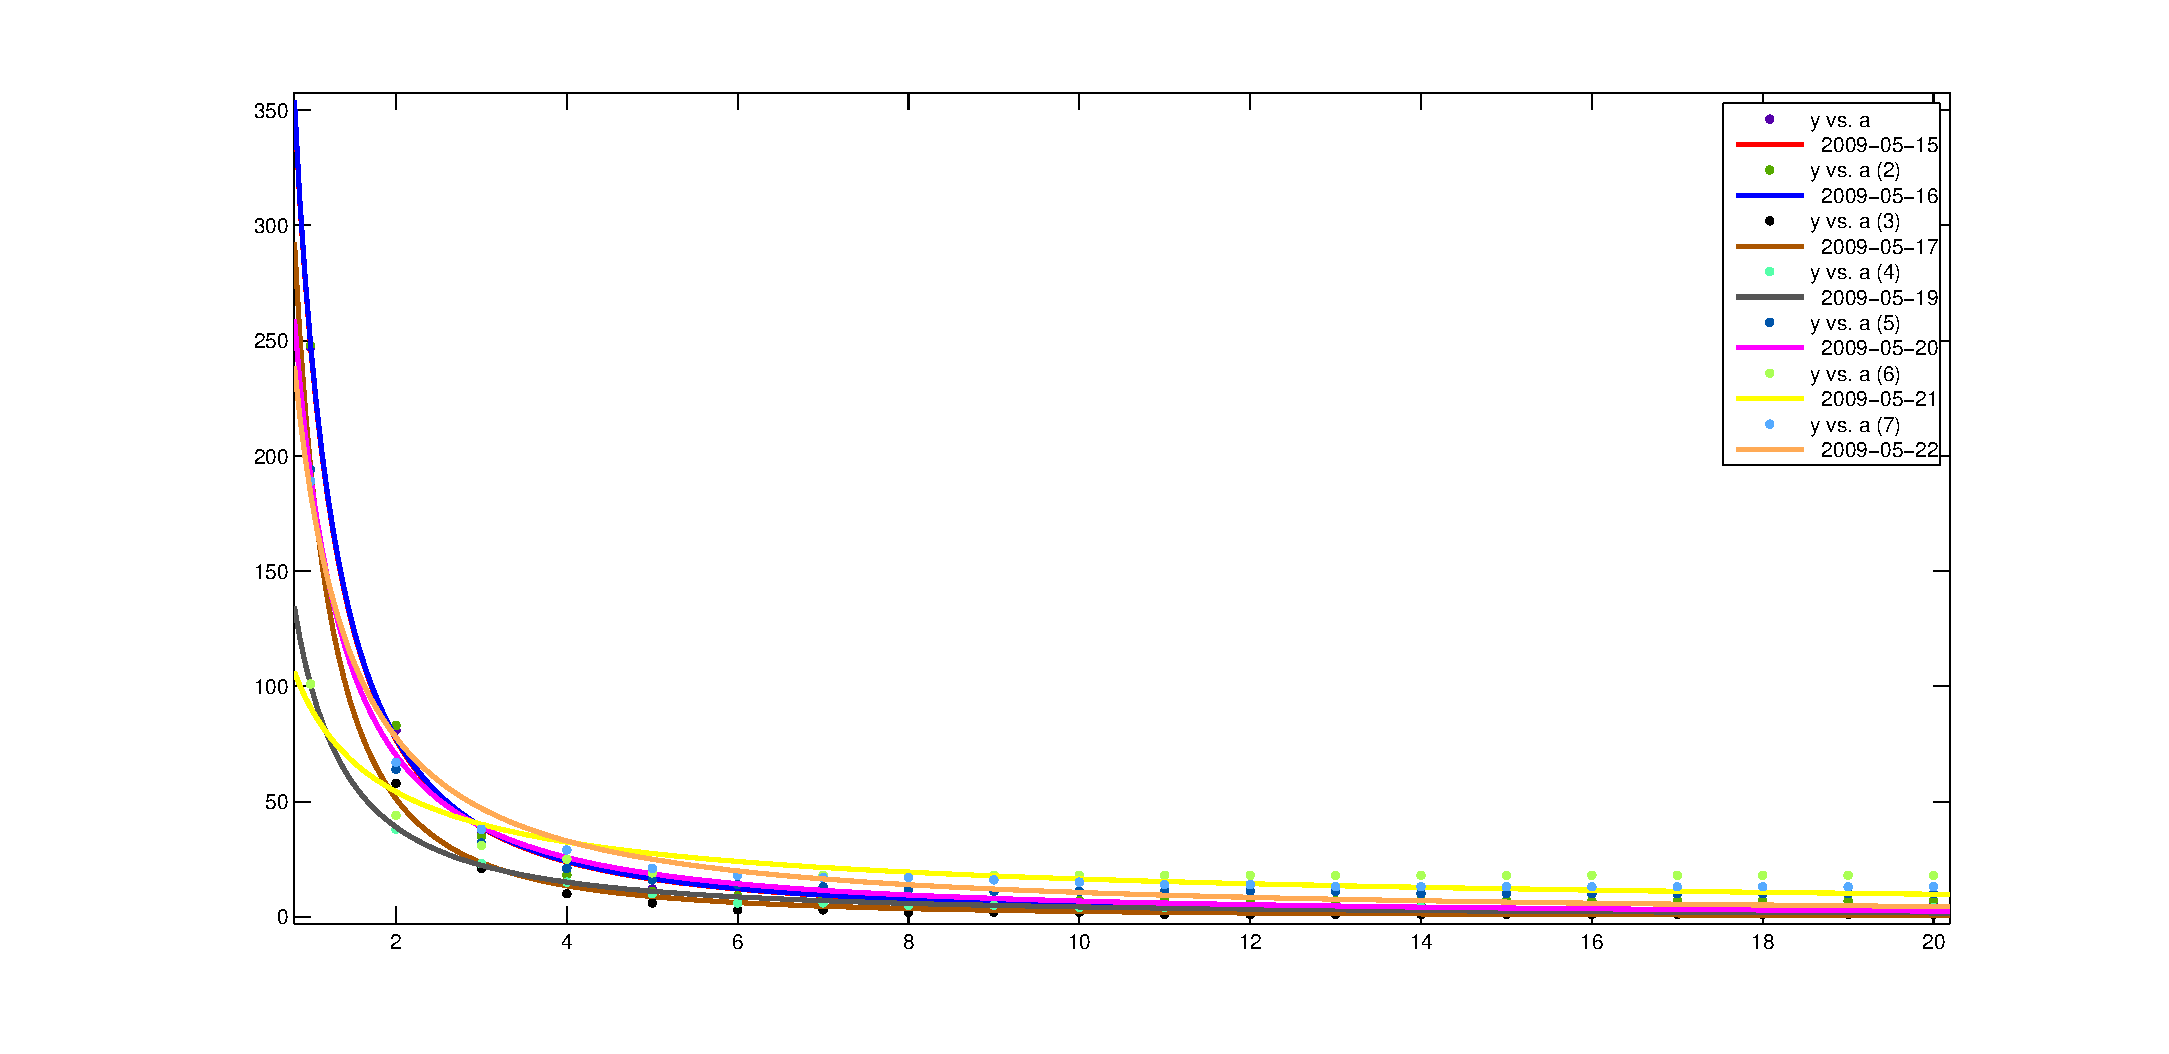
\includegraphics[scale=0.3]{plot3/plot3}
\caption{Plots of Number of boxes($N_B$) vs Length of Box($l_B$) for days 15-21.}
\end{figure}
\begin{figure}
\centering
\includegraphics[scale=0.3]{plot4/plot4}
\caption{Plots of Number of boxes($N_B$) vs Length of Box($l_B$) for days 22-28.}
\end{figure}
\begin{figure}
\centering
\includegraphics[scale=0.3]{plot5/plot5}
\caption{Plots of Number of boxes($N_B$) vs Length of Box($l_B$) for days 29-35.}
\end{figure}
\begin{figure}
\centering
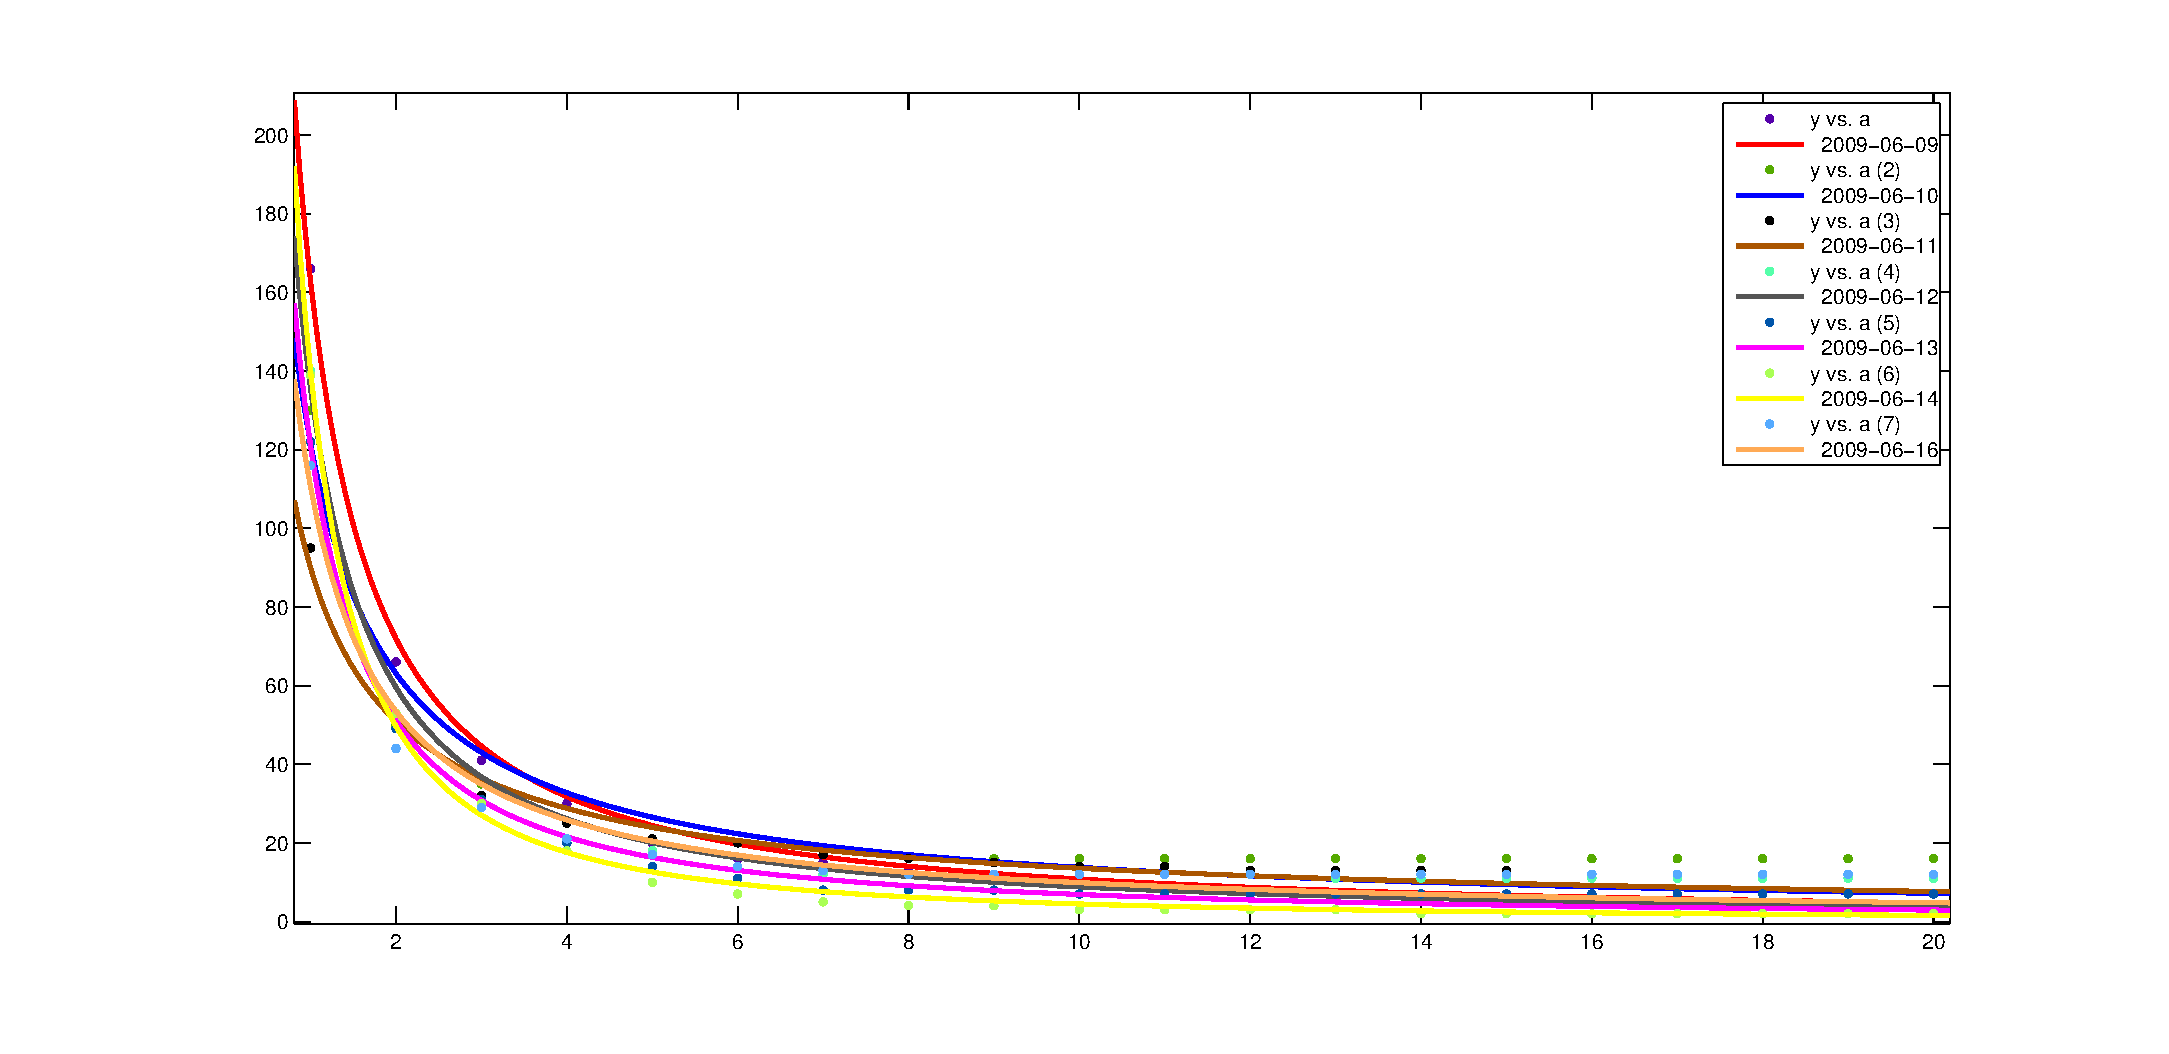
\includegraphics[scale=0.3]{plot6/plot6}
\caption{Plots of Number of boxes($N_B$) vs Length of Box($l_B$) for days 36-42.}
\end{figure}
\begin{figure}
\centering
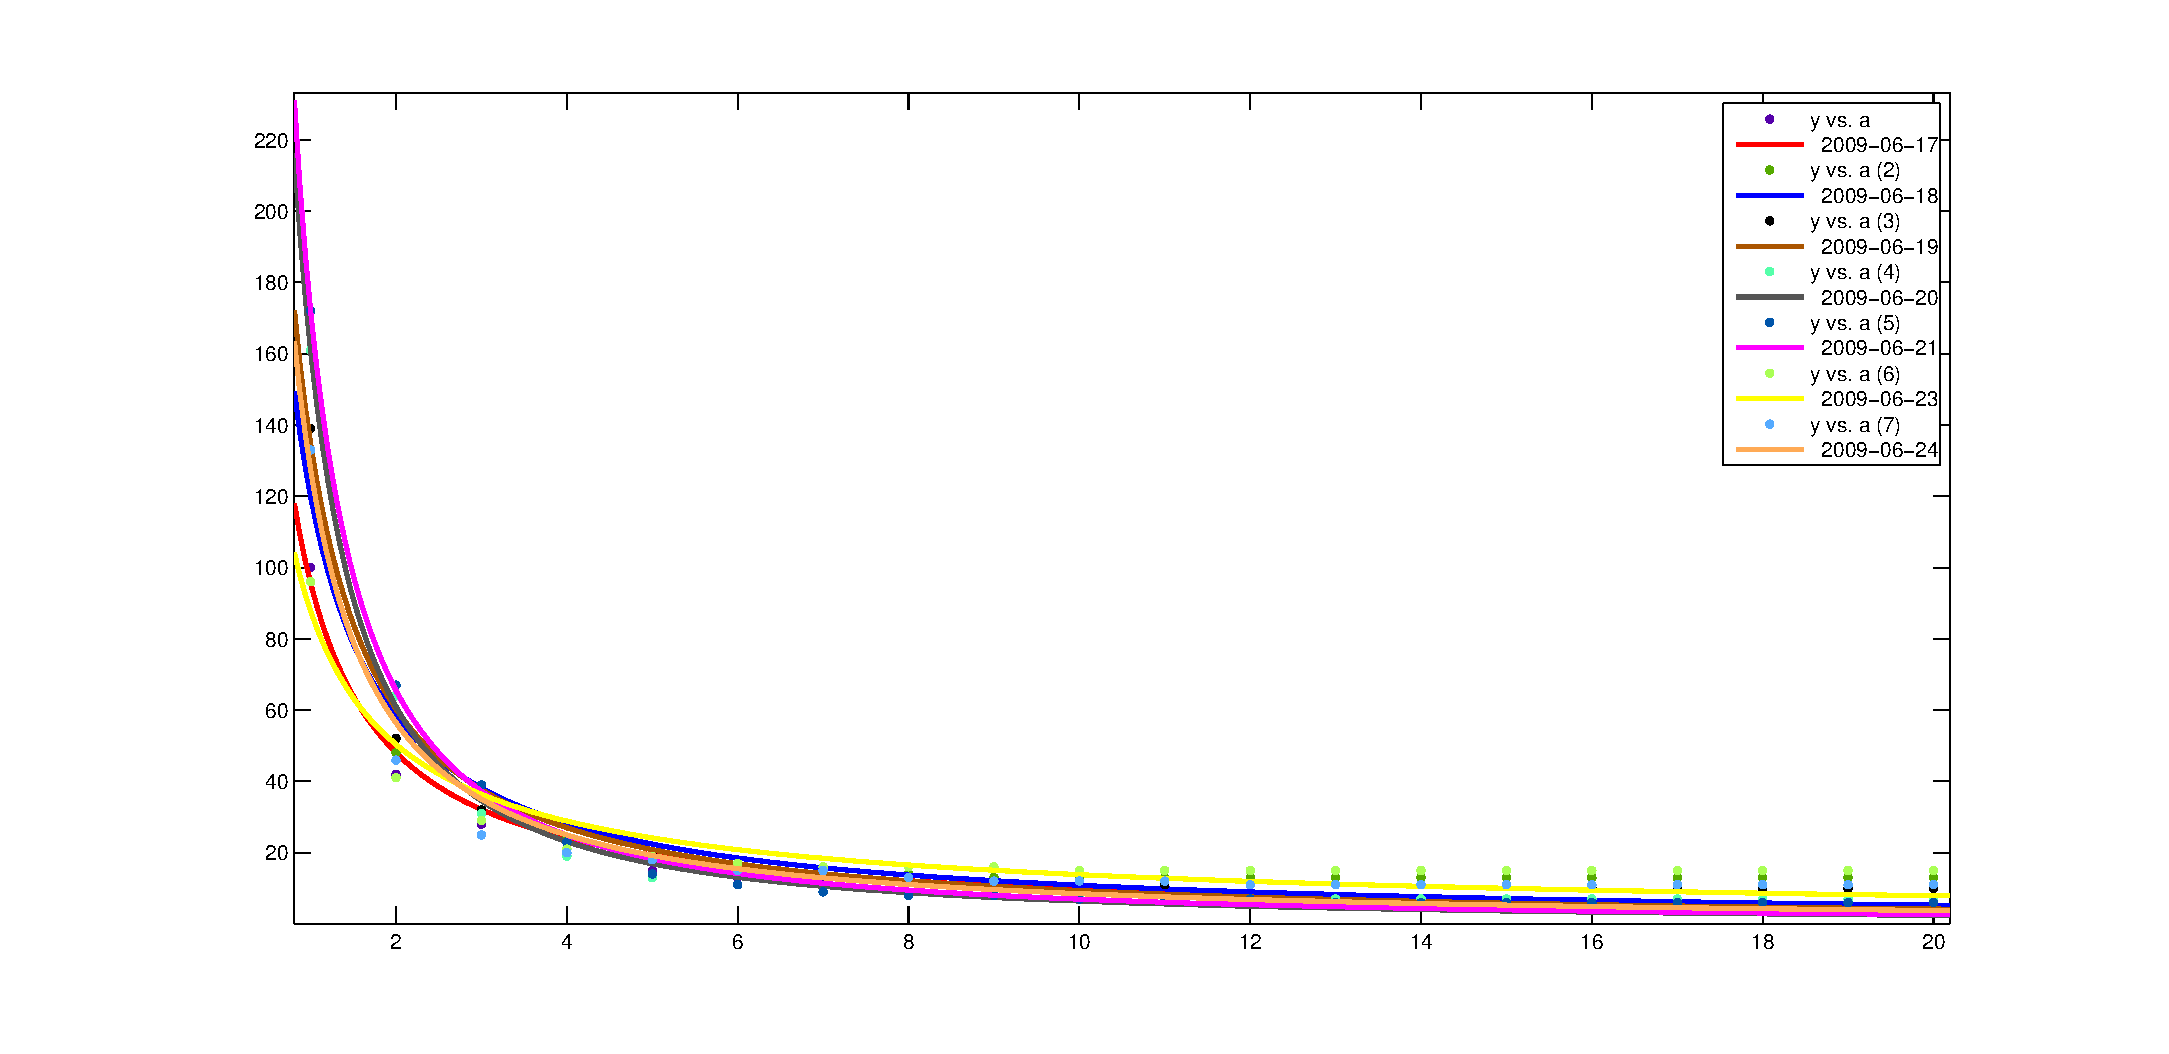
\includegraphics[scale=0.3]{plot7/plot7}
\caption{Plots of Number of boxes($N_B$) vs Length of Box($l_B$) for days 43-49.}
\end{figure}
\begin{figure}
\centering
\includegraphics[scale=0.3]{plot8/plot8}
\caption{Plots of Number of boxes($N_B$) vs Length of Box($l_B$) for days 50-56.}
\end{figure}
\begin{figure}
\centering
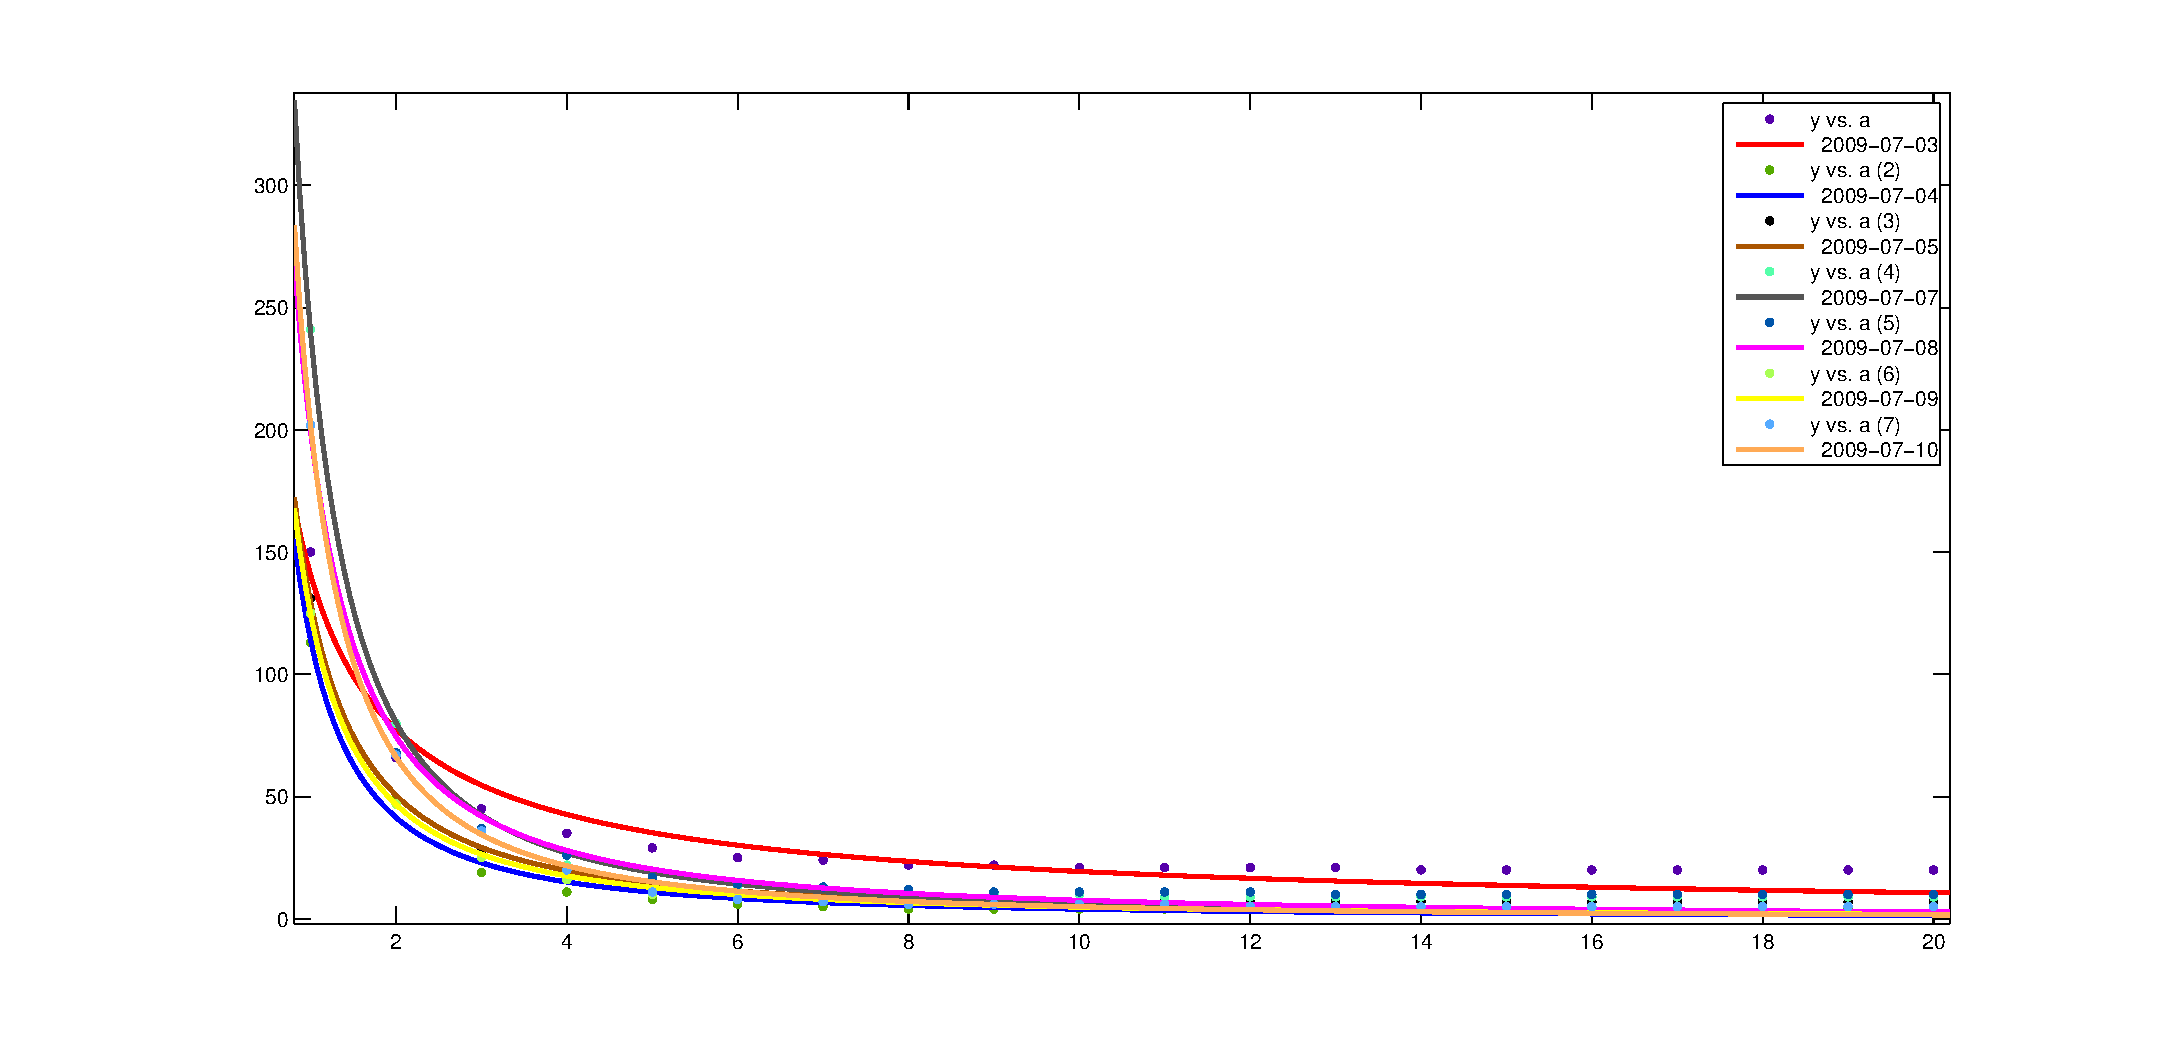
\includegraphics[scale=0.3]{plot9/plot9}
\caption{Plots of Number of boxes($N_B$) vs Length of Box($l_B$) for days 57-63.}
\end{figure}
\begin{figure}
\centering
\includegraphics[scale=0.3]{plot10/plot10}
\caption{Plots of Number of boxes($N_B$) vs Length of Box($l_B$) for days 64-69.}
\end{figure}
\begin{figure*}
\centering
\includegraphics[scale=0.3]{fd/fd_plot}
\caption{variation of Fractal Dimension($d_B$) w.r.t. time($t$)(in days).}
\end{figure*}


\begin{thebibliography}{9}

\bibitem{Ref1}
Ref1

\bibitem{Ref2}
Ref2

\end{thebibliography}

\end{document}